\section{Coding Problems (50 points)}
\begin{notebox}
In this section, we will be implementing, training, and evaluating the neural networks with the image data. Different from the last homework, where we require you to implement the code with Numpy only, the coding problems for this homework will be all about using the amazing machine learning and deep learning libraries. There are two coding problems in total. The first one is a 25-point (warm-up) problem, where you are asked to implement an MLP model to deal with the image classification problem with Keras. The second task requires you to implement a hand-crafted CNN model with PyTorch. We recommend you to run the coding problems on the Google Colab\footnote{\url{https://colab.research.google.com/notebooks/welcome.ipynb?hl=zh-cn}} platform. \textit{\textbf{The links to your colab notebooks should be provided in the following solution box.}}
\end{notebox}

\begin{soln}{height=6cm}
\begin{itemize}
    \item Link to problem 2.1: \url{YOUR ANSWER HERE}
    \item Link to problem 2.2: \url{YOUR ANSWER HERE}    
\end{itemize}
\end{soln}

\clearpage
\subsection{Image Classification with MLP (25 points)}
In this problem, you are asked to implement an MLP to perform an image classification task. The following requirements shall be met to get the full 25 points.
\begin{itemize}
    \item The dataset should be the full MNIST\footnote{\url{http://yann.lecun.com/exdb/mnist/}} dataset;
    \item The data should be flattend and properly normalized before fed into the MLP; \\
    HINT: \textit{tf.keras.datasets.mnist.load\_data()}\footnote{\url{https://keras.io/api/datasets/mnist/}}
    \item Use the \textbf{Sequential} model in Keras;\\
    HINT: \textit{tf.keras.Sequential()}\footnote{\url{https://keras.io/api/models/sequential/}}
    \item Use the idea of validation to tune your model;
    \item Try at least two regularization methods we introduced during lecture:
    \begin{itemize}
        \item L1/L2 regularization: \textit{tf.keras.regularizers}\footnote{\url{https://keras.io/api/layers/regularizers/}}
        \item Dropout: \textit{tf.keras.layers.Dropout()}\footnote{\url{https://keras.io/api/layers/regularization_layers/dropout/}}
        \item Data augmentation: \textit{tf.keras.preprocessing.ImageDataGenerator()}\footnote{\url{https://www.tensorflow.org/api_docs/python/tf/keras/preprocessing/image/ImageDataGenerator}}
        \item Early stopping: \textit{tf.keras.callbacks.EarlyStopping()}\footnote{\url{https://keras.io/api/callbacks/early_stopping/}}
    \end{itemize}
    \item Try at least two optimizers we introduced during lecture: \textit{tf.keras.optimizers} \footnote{\url{https://keras.io/api/optimizers/}}
        \begin{itemize}
        \item SGD
        \item Momentum
        \item Adam
    \end{itemize}
\end{itemize}

\clearpage
\begin{questions}
    \question[2] Your code of data pre-processing (including loading the data, train-val split, and data normalization):
    
    \begin{soln}{height=3cm}
    %%%%%%%%% YOUR SOLUTION HERE %%%%%%%
    \end{soln}
    
    \question[5] Your code of Keras \textbf{Sequential} model definition:
    
    \begin{soln}{height=15cm}
    %%%%%%%%% YOUR SOLUTION HERE %%%%%%%
    \end{soln}
    
    \clearpage
    \question[9] Your results of trying out different regularization techniques (include training and validation loss curves, and your explanation):
    
    \begin{soln}{height=20cm}
    %%%%%%%%% YOUR SOLUTION HERE %%%%%%%
    \end{soln}
    
    \clearpage
    \question[9] Your results of trying out different optimizers (include training and validation loss curves, and your explanation):
    
    \begin{soln}{height=20cm}
    %%%%%%%%% YOUR SOLUTION HERE %%%%%%%
    \end{soln}
\end{questions}


\clearpage
\subsection{Image Classification with CNNs (25 points)}
In this problem, you are asked to implement a CNN to perform an image classification task. The following requirements shall be met to get the full 25 bonus points.
\begin{itemize}
    \item The dataset should be the full CIFAR10\footnote{\url{https://www.cs.toronto.edu/~kriz/cifar.html}} dataset: \textit{torchvision.datasets.CIFAR10}\footnote{\url{https://pytorch.org/vision/stable/generated/torchvision.datasets.CIFAR10.html}}
    \item Use the PyTorch framework for training the model.
    \item Use the \textbf{DataLoader} to iterate through your dataset.\footnote{\url{https://pytorch.org/docs/stable/data.html}}
    \item Define the CNN model inheriting the \textbf{torch.nn.Module}\footnote{\url{https://pytorch.org/docs/stable/generated/torch.nn.Module.html}}
    \item Construct the base convolutional neural network according to the PyTorch tutorial\footnote{\url{https://pytorch.org/tutorials/beginner/blitz/cifar10_tutorial.html}}. The structure of the base convolutional neural network is: 
    \begin{figure}[h]
        \centering
        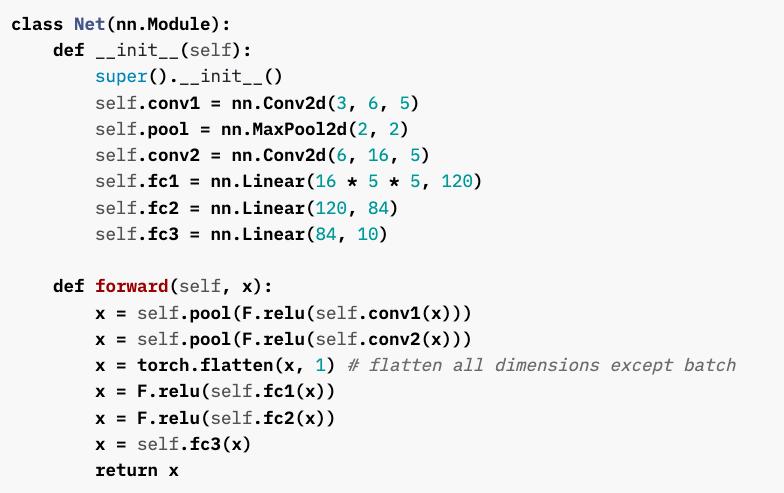
\includegraphics[width=0.7\textwidth]{Homework1/figures/base-cnn.png}
    \end{figure}
    \item Compare the difference between the base model with and without the ReLU activation.
    \item Replace the Pooling layer with the convolutional layer that results in the same output feature map size, and compare the performances between them. 
    \item Make the base CNN deeper and compare their performance.
\end{itemize}

\clearpage
\begin{questions}
    
    \question[2] Your code of \textbf{DataLoader} and iterating the \textbf{DataLoader}:
    
    \begin{soln}{height=20cm}
    %%%%%%%%% YOUR SOLUTION HERE %%%%%%%
    \end{soln}
    
    \clearpage
    \question[4] Report the base CNN's performance (including training and validation losses, training, validation and test accuracy). What's your conclusion about the base CNN model?
    
    \begin{soln}{height=20cm}
    %%%%%%%%% YOUR SOLUTION HERE %%%%%%%
    \end{soln}
    
    \clearpage
    \question[5] Remove the ReLU activation inside the base CNN model and compare their performances (including training and validation losses, training, validation and test accuracy). What's your conclusion?
    
    \begin{soln}{height=20cm}
    %%%%%%%%% YOUR SOLUTION HERE %%%%%%%
    \end{soln}
    
    \clearpage
    \question[7] Replace the Pooling layer with the convolutional layer that results in the same output feature map size, and compare the performances between them (including training and validation losses, training, validation and test accuracy). What's your conclusion?
    
    \begin{soln}{height=20cm}
    %%%%%%%%% YOUR SOLUTION HERE %%%%%%%
    \end{soln}
    
    \clearpage
    \question[7] Make the model deeper and compare the performances between them (including your model structure, training and validation losses, training, validation and test accuracy). What's your conclusion?
    
    \begin{soln}{height=20cm}
    %%%%%%%%% YOUR SOLUTION HERE %%%%%%%
    \end{soln}
    
    \clearpage
    \question[10] BONUS: If your currently attained best model is underfitting, try to alter its structure to overfit, otherwise try some regularization techniques. Report the results and what's your conclusion?
    
    \begin{soln}{height=20cm}
    %%%%%%%%% YOUR SOLUTION HERE %%%%%%%
    \end{soln}
\end{questions}